%!TEX root = ../ecdsa.tex

\chapter{Grundlagen} \label{sec:basics}

%%%%%%%%%%%%%%%%%%%%%%%%%%%%%%%%%%%%%%%%%%%%%%%%%%%%%%%%%%%%%
\section{Gruppen und Endliche Körper}

Eine abelsche Gruppe im mathematischen Sinn ist ein Tupel $(G,\circ)$ aus einer nicht-leeren Menge G und einer darauf definierten inneren Verknüpfung $\circ$ (vgl. \cite{puttmann}, S. 11f). Hierbei entspricht die innere Verknüpfung einer Abbildung 
\begin{center}
$ \circ: X \times X \to X $
\end{center}
die jedem Paar $(x_1,x_2)$ aus Elementen der Menge X ein Element $x_1 \circ x_2$ zuordnet. Außerdem sind folgende Bedingungen auf der Struktur einer Gruppe definiert: \\

\begin{enumerate}
  \item Menge $G$ ist abgeschlossen, d.h. für alle $a,b \in G$ gilt, dass auch jede Verknüpfung $a \circ b$ ein Element von $G$ ist. 
  \item Assoziativgesetz: $ \forall a,b,c \in G: (a \circ b) \circ c = a \circ (b \circ c) $
  \item Kommutativgesetz: $ \forall a,b \in G: a \circ b = b \circ a $
  \item Neutrales Element: $ \forall a \in G: a \circ e = e \circ a = a$
  \item Inverses Element: $ \forall a \in G: a \circ a^{-1} = a^{-1} \circ a = e$\\
\end{enumerate}

Ein Beispiel für eine so definierte abelsche Gruppe entspricht der Menge der ganzen Zahlen $\mathbb{Z}$ mit der Addition als Verknüpfung $(\mathbb{Z},+)$. Die Anzahl der Elemente einer Gruppe wird als Ordnung bezeichnet, welche für die ganzen Zahlen unendlich ist. In der Kryptographie kommen jedoch stets Gruppen mit einer endlichen Anzahl von Elementen zum Einsatz, bei denen also die Ordnung der Gruppe beschränkt ist. 
\\ \\
Eine besondere Form endlicher Gruppen bilden zyklische Gruppen, die ein Element $g$ besitzen, aus dem alle anderen Elemente der Gruppe durch Verknüpfungen $\circ$ erzeugt werden können. Das Element $g$ ist das sog. Generatorelement der zyklischen Gruppe $(G',\circ)$.
\\ \\
Ein Körper ist eine Erweiterung von abelschen Gruppen und als Tripel $(K,+,\cdot)$ definiert, welche zu einer nicht-leeren Menge $K$ die inneren Verknüpfungen Addition und Multiplikation beschreibt. Folgende Bedingungen werden dabei erfüllt (vgl. \cite{puttmann}): \\

\begin{enumerate}
  \item Die Menge $K$ bildet durch die additive Verknüpfung $+$ eine abelsche Gruppe
mit 0 als neutralem Element
  \item Die Menge $K\setminus\{0\}$, d. h. $K$ ohne das Element 0, bildet durch die multiplikative Verknüpfung $\cdot$ ebenfalls eine abelsche Gruppe mit 1 als neutralem Element
  \item Distributivgesetz: $ \forall a,b,c \in K: c \cdot (a + b) = c \cdot a + c \cdot b $ \\
\end{enumerate}

Unter einem Endlichen Körper oder Galoiskörper versteht man einen Körper mit endlich vielen Elementen, der oft auch als Restklassenkörper bezeichnet wird. Ein Beispiel dafür sind Primkörper mit Primzahl $p$ und den Verknüpfungen \textit{Addition modulo p} und \textit{Multiplikation modulo p}: $\mathbb{Z}_p = \{0,1,2,3,\cdots,p-1\}$. 
\\ \\
Galoiskörper werden mit $GF(p)$ abgekürzt, wobei $p$ eine Primzahl sein muss und für die Anzahl der Elemente im Feld steht. $GF(p)$ repräsentiert damit einen Körper der Restklasse ganzer Zahlen modulo $p$. Durch die mathematischen Eigenschaften dieser Struktur eignen sie sich besonders für den Einsatz in der Kryptographie.

%%%%%%%%%%%%%%%%%%%%%%%%%%%%%%%%%%%%%%%%%%%%%%%%%%%%%%%%%%%%%
\section{Elliptische Kurven} 
\label{sec:ell}

Eine elliptische Kurve $E$ über einem Körper $K$ ist eine nicht-singuläre\footnote{Nicht-singulär: keine Knoten, keine Spitzen, keine ``Einsiedler'' (isolierte Punkte)} Kurve (vgl. Abb. \ref{fig:ellkurve}\footnote{Quelle: \url{https://upload.wikimedia.org/wikipedia/de/3/30/Ell\_kurve.png}}), definiert als Menge aller Punkte $(x,y)$ mit $x,y \in K$, für die gilt $F(x,y)=0$ zusammen mit einem ``Punkt in der Unendlichkeit'' O (vgl. \cite{grebe}, S.25).
\\ \\
Eine elliptische Kurve über ein endliches Feld $F_p$ kann mit Hilfe der Weierstraß-Gleichung in Normalform wie folgt definiert werden:

% E:y2+a1xy+a3 y=x3+a2x2+a4x+a6
\begin{center}
$E(K): y^2 + a_1 x y + a_3 y = x^3 + a_2 x^2 + a_4 x + a_6 $
\end{center}

Die Parameter $a_1 \dots a_6$ legen fest, welche Form die elliptische Kurve annimmt und sind Elemente des Feldes $F_p$. Sie werden durch die Domain-Parameter festgelegt. 

\begin{figure}[H]
	\centering
   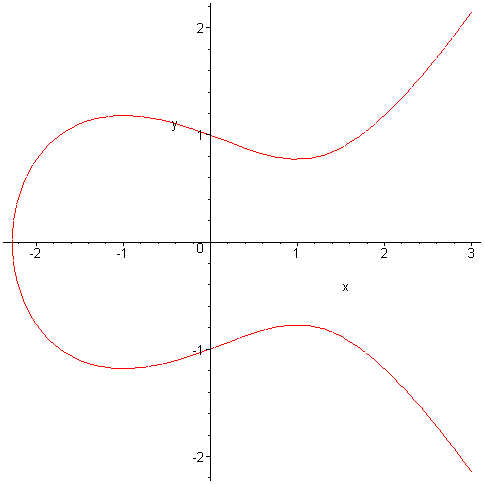
\includegraphics[width=0.60\textwidth]{bilder/ellkurve}
	\caption{Graph einer Elliptischen Kurve}
	\label{fig:ellkurve}
\end{figure}

Über eine Reihe von Vereinfachungen lässt sich die Weierstraß-Gleichung auf die folgende Formel reduzieren:  % y2 mod p=x3+ax+b mod p 
\begin{center}
$ y^2 \bmod p = x^3 + a x + b \bmod p $
\end{center}

Damit eine elliptische Formel in der Kryptographie eingesetzt werden kann, muss zusätzlich die nachfolgende Bedingung gelten. Sie folgt aus der nicht-singulären Eigenschaft von E, also Diskriminante $\ne$ 0 (Herleitung und Beweis siehe \cite{grebe}, S. 28ff):
%4a3+ 27b2 mod p 0
\begin{center}
$ 4 a^3 + 27 b^2 \bmod p \ne 0, $ mit $ a,b \in K $
\end{center}

Entsprechend wie bei endlichen Körpern ist die Ordnung auf einer zyklischen Untergruppe $U_P$ von $E(F_P)$ definiert (vgl. \cite{grebe}, S. 35):
\begin{center}
$ U_P := \{ k P | k \in \mathbb{Z} \}$
$k_0 P = P + P + \cdots + P = O, $ mit $ k_0 > 0$
\end{center}

\subsection{ECC-Operationen}
Auf elliptischen Kurven sind eine Reihe von Operationen definiert. Dazu zählen die Punktaddition, Punktmultiplikation und die Punktdopplung als Spezialfall der Punktaddition.

\begin{figure}[H]
	\centering
	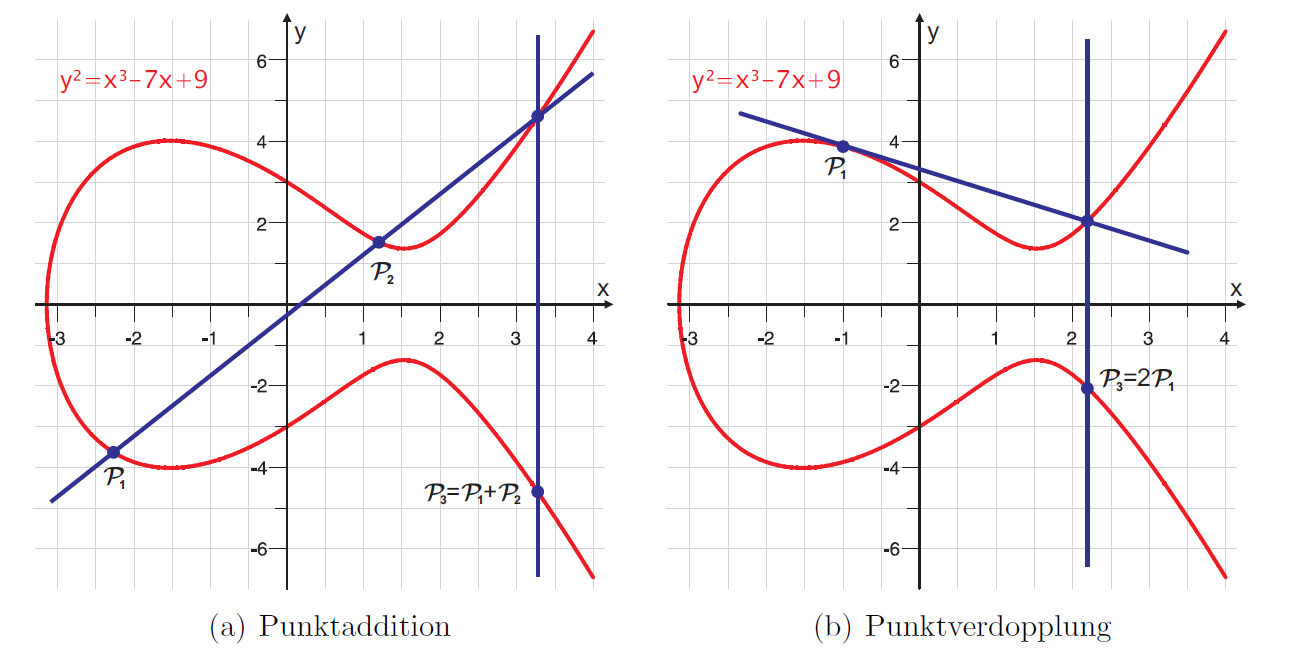
\includegraphics[width=\textwidth]{bilder/p-addition}
	\caption{Arithmetische Operationen auf einer elliptischen Kurve}
	\label{fig:padd}
\end{figure}

Die als Punktaddition bezeichnete arithmetische Operation verknüpft zwei verschiedene Punkte ($P \ne Q$) auf der Kurve miteinander. \\

$R = P + Q$ \\
$s = \frac{p_y-q_y}{p_x-q_x} \mod p$ \\
$r_x = s^2 - p_x - q_x \mod p$ \\
$r_y = s(p_x-r_x)-p_y \mod p$ \\

Wenn die beiden Punkte gleich sind (also $R = P_1 + P_2 = 2 P_1$), wird diese Operation Punktverdopplung genannt (vgl. \cite{puttmann}, S. 16f). \\

$R=P+P$ \\
$s=p_x + \frac{p_x}{p_y} \mod p$ \\  
$r_x=s^2 + s + a \mod p$ \\  
$r_y={p_x}^2 + s{r_x} + r_x \mod p$ \\

Beide Operationen lassen sich mittels Sekanten- bzw. Tangentenmethode auf einer elliptischen Kurve darstellen (s. Abb. \ref{fig:padd}\footnote{Quelle: s. \cite{puttmann}, S. 17}). 
\\ \\
Die Punkt-Multiplikation führt eine k-fache Punktaddition durch. \\

$R = k A \mod p$

\subsection{Koblitz-Kurven}
Eine besondere Form der elliptischen Kurven sind \texttt{Koblitz}-Kurven (engl. Anomalous Binary Curves) über das endliche Feld $F_{2^m}$, deren Kurvengleichung ausschließlich die Koeffizienten ``0'' und ``1'' enthalten. In kryptographischen Protokollen werden häufig Koblitz-Kurven der folgenden Formen verwendet (vgl. \cite{guide}, Kap. 3.4):

\begin{center}
$E_0 : y^2 + x y = x^3 + 1 $ \\
$E_1 : y^2 + x y = x^3 + x^2 + 1 $
\end{center}

Der große Vorteil dieser Kurven ist, dass Algorithmen zur Punktmultiplikation prinzipiell ohne Punktverdopplung auskommen können (s. \cite{guide}, S. 114). Darüberhinaus eignen sich Koblitz-Kurven besonders für den Einsatz in Hardwaresystemen, da für sie allgemein hocheffiziente Algorithmen für Punktarithmetik existieren, wohingegen sich klassische Kurven $F_P$ eher für Softwaresysteme eignen. In der Praxis wurden bisher keine Sicherheitsunterschiede festgestellt.

%%%%%%%%%%%%%%%%%%%%%%%%%%%%%%%%%%%%%%%%%%%%%%%%%%%%%%%%%%%%%
\section{Das Diskrete Logarithmus-Problem} \label{sec:dlp}

Das Problem des diskreten Logarithmus in endlichen Körpern besteht darin, dass die Lösung eines solchen Logarithmus viel schwieriger ist, als die Umkehrfunktion, also die diskrete Exponentialfunktion. Die Sicherheit von auf elliptischen Kurven basierenden kryptographischen Verfahren beruht auf diesem mathematischen Problem. 
\\ \\
Definition nach \cite{baum} (S. 6):
\begin{itemize}
	\item \textbf{Voraussetzungen:}\\
	Sei $(G,\cdot)$ eine multiplikative Gruppe, $x \in G$ ein Element der Ordnung $n$ und $y \in \left \langle x \right \rangle$.
	\item \textbf{Problem:}\\
	Man berechnet $a$ mit $(0 \le a \le n-1)$, sodass $x^a = y$. \\
	``$a$'' wird diskreter Logarithmus von $y$ zur Basis $x$ genannt. \\
\end{itemize}

Umgangssprachlich wird eine solche Funktion \textit{Einwegfunktion} genannt. Dabei entspricht der diskrete Logarithmus einer Funktion $f: M \implies N$, wenn für ``fast alle'' Bilder $y \in N$ kein Urbild $x \in M$ mit $f(x) = y$ effizient bestimmbar ist (vgl. \cite{diskrlog}, S. 54).
\\ \\
Bezogen auf eine elliptische Kurve (engl. Elliptic Curve Discrete Logarithm Problem, ECDLP) $E(GF(2^n))$ bedeutet das, dass die Skalarmultiplikation $Q = k P$ für eine natürliche Zahl $k$ und einen Punkt $P$ nach der Kurvengleichung sehr einfach zu berechnen ist ($Q$ ist die $(k-1)$-fache Addition mit $P$), es aber \textit{schwierig} ist, aus zwei vorgegebenen Punkten $Q, P \in E(GF(2^n))$ wieder die Zahl $k$ zu ermitteln (vgl. \cite{puttmann}, S. 17f).

%%%%%%%%%%%%%%%%%%%%%%%%%%%%%%%%%%%%%%%%%%%%%%%%%%%%%%%%%%%%%
\section{Digitale Signaturen} \label{sec:digsig}

Eine digitale Signatur nutzt ein asymmetrisches Verschlüsselungsverfahren, um eine schlüsselabhängige Prüfsumme eines Dokuments zu erzeugen (vgl. \cite{wolf}). Der Schlüssel zum Überprüfen einer Signatur ist öffentlich, während der Schlüssel zum Signieren geheim gehalten werden muss. Somit kann jeder ein digital ``unterschriebenes'' Dokument auf seine Echtheit überprüfen bzw. verifizieren.

\begin{figure}[H]
	\centering
   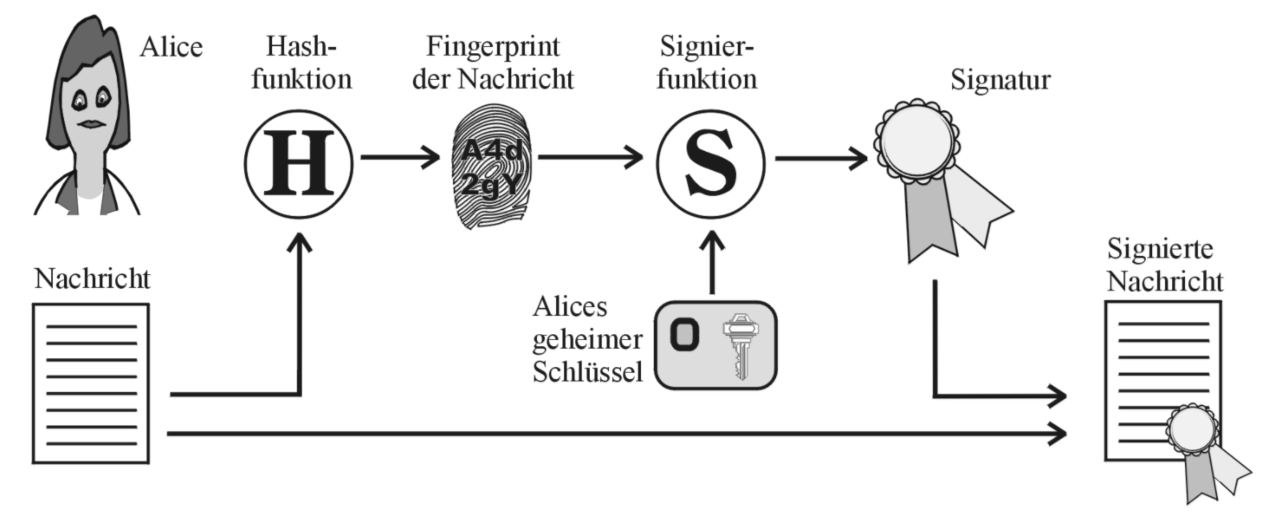
\includegraphics[width=0.80\textwidth]{bilder/digisig}
	\caption{Erzeugung einer Digitalen Signatur}
	\label{fig:digisig}
\end{figure}

Abbildung \ref{fig:digisig}\footnote{Quelle: \url{https://www.informatik.tu-darmstadt.de/BS/Lehre/Sem98\_99/T11/index.html}} zeigt den Vorgang der Erzeugung einer Signatur. Die im Bild zu sehende ``Signierfunktion'' muss eine asymmetrische Verschlüsselung sein und entspricht dem in dieser Arbeit implementierten ECDSA-Algorithmus.

%%%%%%%%%%%%%%%%%%%%%%%%%%%%%%%%%%%%%%%%%%%%%%%%%%%%%%%%%%%%%
\section{Der ECDSA Algorithmus}
\label{ecdsa-algo}
%Beim \textit{Elliptic Curve Digital Signature Algorithm} ist die Multiplikation mit einem Punkt auf der elliptischen Kurve die rechnerisch aufwändigste Operation (vgl. \cite{hwimp}), genauer die Skalarmultiplikation $k P$, wobei $k$ eine positive Ganzzahl und $P$ ein Punkt auf der Kurve ist. \\

\subsection{Schlüsselgenerierung \& Domain Parameter}

Beim \textit{Elliptic Curve Digital Signature Algorithm} (ECDSA) wird von einer Partei A ein Schlüssel generiert und damit die Signatur zu einer Nachricht erstellt. Eine andere Partei B nutzt den öffentlichen Schlüssel von A und verifiziert damit die Echtheit der Nachricht von A anhand der Signatur. Folgende Definition (vgl. \cite{hwimp}) berechnet die Schlüssel von A: \\

\begin{enumerate}
%Key generation : (A)
\item Wähle ein zufälliges $d$ aus $[1, n-1]$.
\item Berechne $Q = dP$ .
\item Der öffentliche Schlüssel von A entspricht $Q$; der private Schlüssel ist $d$. \\
\end{enumerate}

Der private Schlüssel $d$ ist hierbei eine positive ganze Zahl. Der Parameter $n$ entspricht der Ordnung des Basis-Punkts $P$. Die Domain Parameter werden allgemein angegeben als $D = (q,FR, S,a,b, P,n,h)$ und werden definiert als (vgl. \cite{guide}, S. 172): \\

\begin{itemize}
\item $q$: Ordnung der Kurve.
\item $FR$: Repräsentation der Elemente in $F_q$.
\item $S$: \textit{Seed}, falls die Kurve zufällig generiert ist.
\item $a,b \in F_q$: Koeffizienten, die die elliptische Kurve beschreiben.
\item $P = (x_P,y_P) \in E(F_q)$: Basis-Punkt der elliptischen Kurve.
\item $n$: Ordnung von $P$.
\item $h$: \textit{Ko-Faktor} $h = \#E(F_q)/n$.
\end{itemize}

\subsection{Signatur}
Erstellen der Signatur (vgl. \cite{hwimp}) : (A)

\begin{enumerate}
\item Zufallszahl $k$ im Bereich $[1, n - 1]$ bestimmen.
\item Berechne $k G = (x_1, y_1)$ mit $r = x_1 \pmod{n} $.
\item Wenn $r = 0$ dann zurück zu 1.
\item Berechne $k^{-1} \pmod{n}$.
\item Berechne $s = k^{-1}(SHA-1(m) + dr)\pmod{n}$.
\item Wenn $s = 0$ dann zurück zu 1.
\item Sende $m$ und $(r, s)$ zu B
\end{enumerate}

\subsection{Verifikation}
Verifizierung der Signatur (vgl. \cite{hwimp}) : (B)

\begin{enumerate}
\item Überprüfe das $r$ und $s$ Zahlen in $[1, n - 1]$ sind.
\item Berechne $e = SHA - 1(m)$.
\item Berechne $w = s^{-1}\pmod{n}$.
\item Berechne $u_1 = e * w \pmod{n}$ und $u_2 = r * w \pmod{n}$.
\item Berechne $u_1 P + u_2 Q = (x1, y1)$ und $v = x_1 \pmod{n}$.
\item Wenn $s = 0$ dann zurück zu 1.
\item Akzeptiere die Signatur, wenn $v = r$ gilt.
\end{enumerate}






%%%%%%%%%%%%%%%%%%%%%%%%%%%%%%%%%%%%%%%%%%%%%%%%%%%%%%%%%%%%%
\section{UART-Schnittstelle} \label{sec:iuart}

Bei der UART-Kommunikation (engl. Universal Asynchronous Receiver Transmitter, UART) werden Daten über zwei Pins ausgetauscht. Dabei dient ein Pin dem Empfangen (RX-Pin) und der andere dem Senden (TX-Pin). Zur Übertragung der Daten zwischen zwei UART-Schnittstellen werden die Pins über Kreuz verbunden (vgl. \cite{uart}). Üblicherweise übernimmt ein UART-Hardwaremodul auch die Transformation paralleler Daten in einen sequentiellen Datenstrom und umgekehrt.

\begin{figure}[H]
	\centering
   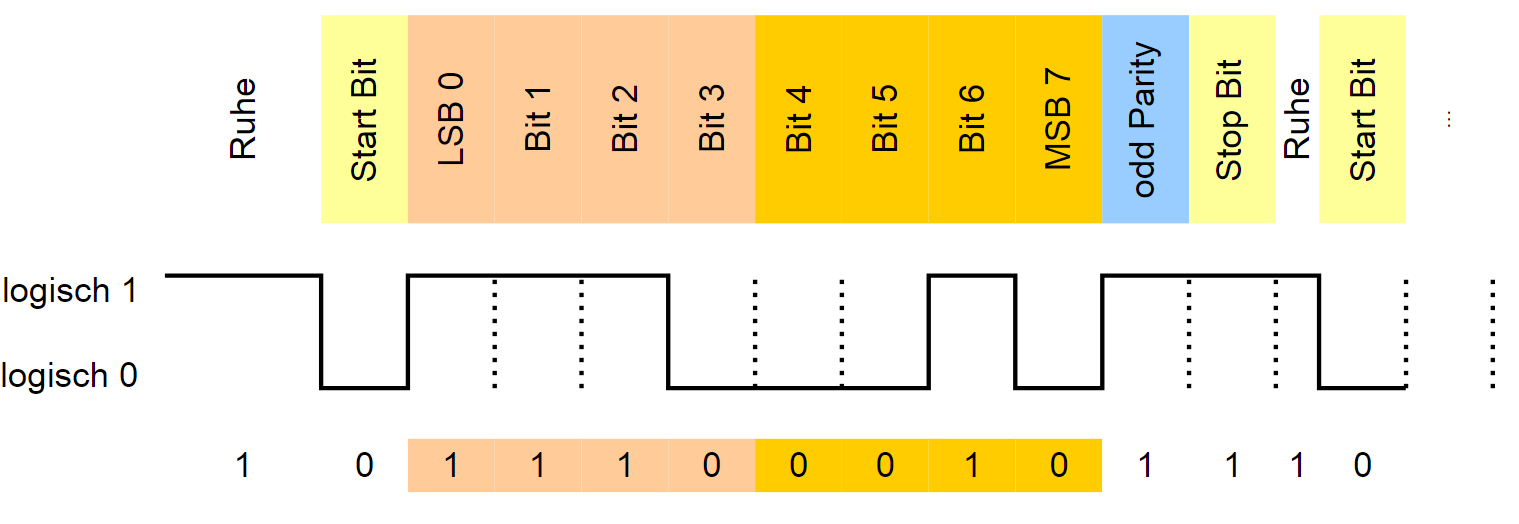
\includegraphics[width=0.90\textwidth]{bilder/uart}
	\caption{Signalübertragung über das UART-Protokoll}
	\label{fig:uart}
\end{figure}

Die Daten werden zu Paketen von meist 8 Bit übertragen, wobei die Sende-Reihenfolge in der Regel vom geringwertigstem Bit (engl. Least Significant Bit, LSB) zum höchstwertigstem Bit (engl. Most Significant Bit, MSB) versendet wird (vgl. Abb. \ref{fig:uart}\footnote{Quelle: \url{https://de.wikipedia.org/wiki/Universal\_Asynchronous\_Receiver\_Transmitter\#/media/File:RS-232_timing.svg}}). Wenn bei einer UART-Verbindung keine Daten übertragen werden, liegt ein ``High''-Pegel an (logisch ``1''). Die Übertragung beginnt mit einem Start-Bit (logisch ``0'') für einen UART-Taktzyklus, wonach die Daten-Bits folgen. Je nach Implementierung kann eine Parität ergänzt werden, die kennzeichnet, ob das Datenpaket eine gerade oder ungerade Anzahl ``1'' enthält. Ein Stop-Bit beendet die Transmission eines Datenpaketes. Ein \textit{UART-Taktzyklus} beschreibt, wie lange die Spannung eines einzelnen Symbols anliegt. Die entsprechende Einheit wird in \textit{Baud} angegeben und entspricht $1 * s^{-1}$. Bei einer Übertragungsrate von 9600 Baud liegt ein Bit also für $1 / 9600s = 104,167 \mu s$ am Ausgang Tx an.

